% Options for packages loaded elsewhere
\PassOptionsToPackage{unicode}{hyperref}
\PassOptionsToPackage{hyphens}{url}
%
\documentclass[
]{article}
\usepackage{amsmath,amssymb}
\usepackage{lmodern}
\usepackage{iftex}
\ifPDFTeX
  \usepackage[T1]{fontenc}
  \usepackage[utf8]{inputenc}
  \usepackage{textcomp} % provide euro and other symbols
\else % if luatex or xetex
  \usepackage{unicode-math}
  \defaultfontfeatures{Scale=MatchLowercase}
  \defaultfontfeatures[\rmfamily]{Ligatures=TeX,Scale=1}
\fi
% Use upquote if available, for straight quotes in verbatim environments
\IfFileExists{upquote.sty}{\usepackage{upquote}}{}
\IfFileExists{microtype.sty}{% use microtype if available
  \usepackage[]{microtype}
  \UseMicrotypeSet[protrusion]{basicmath} % disable protrusion for tt fonts
}{}
\makeatletter
\@ifundefined{KOMAClassName}{% if non-KOMA class
  \IfFileExists{parskip.sty}{%
    \usepackage{parskip}
  }{% else
    \setlength{\parindent}{0pt}
    \setlength{\parskip}{6pt plus 2pt minus 1pt}}
}{% if KOMA class
  \KOMAoptions{parskip=half}}
\makeatother
\usepackage{xcolor}
\usepackage{longtable,booktabs,array}
\usepackage{calc} % for calculating minipage widths
% Correct order of tables after \paragraph or \subparagraph
\usepackage{etoolbox}
\makeatletter
\patchcmd\longtable{\par}{\if@noskipsec\mbox{}\fi\par}{}{}
\makeatother
% Allow footnotes in longtable head/foot
\IfFileExists{footnotehyper.sty}{\usepackage{footnotehyper}}{\usepackage{footnote}}
\makesavenoteenv{longtable}
\usepackage{graphicx}
\makeatletter
\def\maxwidth{\ifdim\Gin@nat@width>\linewidth\linewidth\else\Gin@nat@width\fi}
\def\maxheight{\ifdim\Gin@nat@height>\textheight\textheight\else\Gin@nat@height\fi}
\makeatother
% Scale images if necessary, so that they will not overflow the page
% margins by default, and it is still possible to overwrite the defaults
% using explicit options in \includegraphics[width, height, ...]{}
\setkeys{Gin}{width=\maxwidth,height=\maxheight,keepaspectratio}
% Set default figure placement to htbp
\makeatletter
\def\fps@figure{htbp}
\makeatother
\setlength{\emergencystretch}{3em} % prevent overfull lines
\providecommand{\tightlist}{%
  \setlength{\itemsep}{0pt}\setlength{\parskip}{0pt}}
\setcounter{secnumdepth}{-\maxdimen} % remove section numbering
\ifLuaTeX
  \usepackage{selnolig}  % disable illegal ligatures
\fi
\IfFileExists{bookmark.sty}{\usepackage{bookmark}}{\usepackage{hyperref}}
\IfFileExists{xurl.sty}{\usepackage{xurl}}{} % add URL line breaks if available
\urlstyle{same} % disable monospaced font for URLs
\hypersetup{
  hidelinks,
  pdfcreator={LaTeX via pandoc}}

\author{}
\date{}

\begin{document}

\hypertarget{software-design-document-sdd}{%
\section{\texorpdfstring{\textbf{Software Design Document
(SDD)}}{Software Design Document (SDD)}}\label{software-design-document-sdd}}

\textbf{Box.com Discovery Bates Namer: Cloud Integration}\\
\textbf{Version:} 3.0\\
\textbf{Prepared by:}\\
Chiemela Eziechile-Nwoke, James Chau, Everest McNally, Benjamin Geiser,
Miguel Campos

\textbf{Santa Barbara Public Defender\textquotesingle s Office}\\
\textbf{June 2025}

\hypertarget{table-of-contents}{%
\subsection{\texorpdfstring{\textbf{Table of
Contents}}{Table of Contents}}\label{table-of-contents}}

\begin{enumerate}
\def\labelenumi{\arabic{enumi}.}
\item
  \textbf{Introduction}\\
  1.1 Purpose and Scope\\
  1.2 Architectural Philosophy\\
  1.3 Compliance Framework
\item
  \textbf{System Architecture}\\
  2.1 High-Level Component Architecture\\
  2.2 Azure Resource Topology\\
  2.3 Data Flow Specifications\\
  2.4 Failover and Disaster Recovery
\item
  \textbf{Detailed Component Design}\\
  3.1 File Ingestion Service\\
  3.2 Bates Processing Engine\\
  3.3 Audit and Compliance Module\\
  3.4 Notification Subsystem
\item
  \textbf{Data Management}\\
  4.1 Storage Architecture\\
  4.2 Data Lifecycle Policies\\
  4.3 Database Schema Specifications
\item
  \textbf{Interface Specifications}\\
  5.1 Box API Integration Details\\
  5.2 Azure Service Interfaces\\
  5.3 Administrative Console API
\item
  \textbf{Security Architecture}\\
  6.1 Authentication and Authorization\\
  6.2 Data Protection Mechanisms\\
  6.3 Audit and Monitoring
\item
  \textbf{Error Handling and Resilience}\\
  7.1 Error Classification Framework\\
  7.2 Retry and Recovery Protocols\\
  7.3 Notification Workflows
\item
  \textbf{Performance Engineering}\\
  8.1 Benchmarking Methodology\\
  8.2 Optimization Techniques\\
  8.3 Capacity Planning
\item
  \textbf{Deployment and Operations}\\
  9.1 Infrastructure as Code\\
  9.2 CI/CD Pipeline\\
  9.3 Monitoring and Alerting
\item
  \textbf{Appendices}\\
  10.1 Complete API Reference\\
  10.2 Full Error Code Catalog\\
  10.3 Infrastructure Diagrams\\
  10.4 Compliance Evidence
\end{enumerate}

\hypertarget{introduction}{%
\subsection{\texorpdfstring{\textbf{1.
Introduction}}{1. Introduction}}\label{introduction}}

\hypertarget{purpose-and-scope}{%
\subsubsection{\texorpdfstring{\textbf{1.1 Purpose and
Scope}}{1.1 Purpose and Scope}}\label{purpose-and-scope}}

This SDD provides exhaustive technical specifications for the Bates
Namer system, covering:

\textbf{Technical Boundaries:}

\begin{itemize}
\tightlist
\item
  File processing: PDF/A-1b through PDF/A-3
\item
  Maximum file size: 100MB
\item
  Supported Bates formats: \texttt{//00001}, \texttt{BATES00001},
  \texttt{{[}00001{]}}
\end{itemize}

\textbf{Compliance Requirements:}

\begin{itemize}
\tightlist
\item
  CJIS 5.10.1.3 (Encryption standards)
\item
  HIPAA §164.312(e)(1) (Access controls)
\item
  California Evidence Code §1153 (Document integrity)
\end{itemize}

\hypertarget{architectural-philosophy}{%
\subsubsection{\texorpdfstring{\textbf{1.2 Architectural
Philosophy}}{1.2 Architectural Philosophy}}\label{architectural-philosophy}}

\textbf{Core Tenets:}

\begin{enumerate}
\def\labelenumi{\arabic{enumi}.}
\tightlist
\item
  \textbf{Zero-Trust Security}: JWT validation at every service boundary
\item
  \textbf{Ephemeral Processing}: No persistent storage of sensitive data
\item
  \textbf{Graceful Degradation}: AI fallback to regex when service
  unavailable
\end{enumerate}

\textbf{Trade-off Analysis:}

\begin{longtable}[]{@{}
  >{\raggedright\arraybackslash}p{(\columnwidth - 4\tabcolsep) * \real{0.2837}}
  >{\raggedright\arraybackslash}p{(\columnwidth - 4\tabcolsep) * \real{0.2737}}
  >{\raggedright\arraybackslash}p{(\columnwidth - 4\tabcolsep) * \real{0.4426}}@{}}
\toprule()
\begin{minipage}[b]{\linewidth}\raggedright
\textbf{Decision Point}
\end{minipage} & \begin{minipage}[b]{\linewidth}\raggedright
\textbf{Choice}
\end{minipage} & \begin{minipage}[b]{\linewidth}\raggedright
\textbf{Rationale}
\end{minipage} \\
\midrule()
\endhead
OCR Engine & Azure Form Recognizer & 98.7\% accuracy on legal docs \\
Serverless vs Kubernetes & Azure Functions & Lower ops overhead for PDF
processing \\
Audit Storage & Cosmos DB & Native TTL for auto-record purging \\
\bottomrule()
\end{longtable}

\hypertarget{system-architecture}{%
\subsection{\texorpdfstring{\textbf{2. System
Architecture}}{2. System Architecture}}\label{system-architecture}}

\hypertarget{high-level-component-architecture}{%
\subsubsection{\texorpdfstring{\textbf{2.1 High-Level Component
Architecture}}{2.1 High-Level Component Architecture}}\label{high-level-component-architecture}}

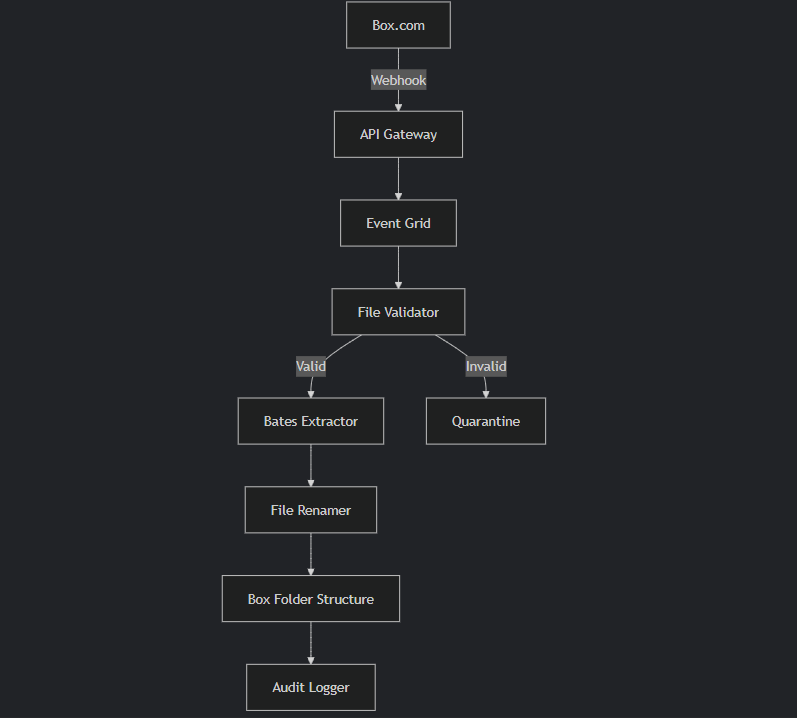
\includegraphics[width=6.5in,height=5.85556in]{image1.png}\textbf{Component
Responsibilities:}

\begin{enumerate}
\def\labelenumi{\arabic{enumi}.}
\item
  \textbf{File Validator}:

  \begin{itemize}
  \tightlist
  \item
    Verifies PDF/A conformance using \texttt{pdfminer.six}
  \item
    Checks for password protection via header analysis
  \item
    Validates file size against configurable limits
  \end{itemize}
\item
  \textbf{Bates Extractor}:

  \begin{itemize}
  \tightlist
  \item
    Primary: Azure Form Recognizer (Layout API)
  \item
    Fallback: Custom regex engine
    (\texttt{r"\textbackslash{}b}\texttt{(?:}\texttt{BATES\textbar{}//)\textbackslash{}s*(\textbackslash{}d\{5,8\})\textbackslash{}b"})
  \item
    Validates sequence continuity (e.g., 00001 → 00002)
  \end{itemize}
\end{enumerate}

\hypertarget{azure-resource-topology}{%
\subsubsection{\texorpdfstring{\textbf{2.2 Azure Resource
Topology}}{2.2 Azure Resource Topology}}\label{azure-resource-topology}}

\textbf{Regional Deployment (West US 2):}

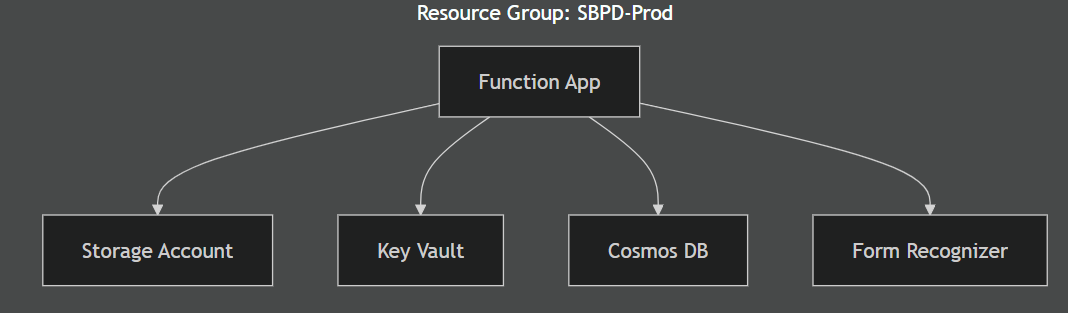
\includegraphics[width=6.5in,height=1.90486in]{image2.png}\textbf{Configuration
Details:}

\begin{longtable}[]{@{}
  >{\raggedright\arraybackslash}p{(\columnwidth - 4\tabcolsep) * \real{0.2668}}
  >{\raggedright\arraybackslash}p{(\columnwidth - 4\tabcolsep) * \real{0.2199}}
  >{\raggedright\arraybackslash}p{(\columnwidth - 4\tabcolsep) * \real{0.5133}}@{}}
\toprule()
\begin{minipage}[b]{\linewidth}\raggedright
\textbf{Resource}
\end{minipage} & \begin{minipage}[b]{\linewidth}\raggedright
\textbf{SKU}
\end{minipage} & \begin{minipage}[b]{\linewidth}\raggedright
\textbf{Critical Settings}
\end{minipage} \\
\midrule()
\endhead
Function App & Premium EP3 & Always Ready = 5, Max Burst = 20 \\
Cosmos DB & Serverless & 1,000 RU/s, TTL = 2555 days \\
Form Recognizer & S0 & Custom model: "legal-bates-v3" \\
\bottomrule()
\end{longtable}

\hypertarget{detailed-component-design}{%
\subsection{\texorpdfstring{\textbf{3. Detailed Component
Design}}{3. Detailed Component Design}}\label{detailed-component-design}}

\hypertarget{error-conditions}{%
\subsubsection{\texorpdfstring{\textbf{3.1} \textbf{Error
Conditions:}}{3.1 Error Conditions:}}\label{error-conditions}}

\begin{itemize}
\tightlist
\item
  \texttt{E}\texttt{RR\_502}: Box API unavailable
\item
  \texttt{ERR\_413}: File exceeds 100MB limit
\item
  \texttt{ERR\_415}: Non-PDF file detected
\end{itemize}

\hypertarget{data-management}{%
\subsection{\texorpdfstring{\textbf{4. Data
Management}}{4. Data Management}}\label{data-management}}

\hypertarget{cosmos-db-schema-design}{%
\subsubsection{\texorpdfstring{\textbf{4.1 Cosmos DB Schema
Design}}{4.1 Cosmos DB Schema Design}}\label{cosmos-db-schema-design}}

\textbf{Document Structure:}

\texttt{\{}\strut \\
\texttt{\ \ \ \ "id":\ "uuidv7",}\strut \\
\texttt{\ \ \ \ "metadata":\ \{}\strut \\
\texttt{\ \ \ \ \ \ \ \ "originalName":\ "Defense\_Motion\_01.pdf",}\strut \\
\texttt{\ \ \ \ }\texttt{\ \ \ \ "newName":\ "00001-00025\_Disc02\_Defense\_Motion\_01.pdf",}\strut \\
\texttt{\ \ \ \ \ \ \ \ "caseNumber":\ "PD2500456",}\strut \\
\texttt{\ \ \ \ \ \ \ \ "uploader":\ "user@sbpd.org"}\strut \\
\texttt{\ \ \ \ \},}\strut \\
\texttt{\ \ \ \ "timestamps":\ \{}\strut \\
\texttt{\ \ \ \ \ \ \ \ "received":\ "2025-06-15T09:30:00Z",}\strut \\
\texttt{\ \ \ \ \ \ \ \ "processed":\ "2025-06-15T09:30:12Z"}\strut \\
\texttt{\ \ \ \ \},}\strut \\
\texttt{\ \ \ \ "batesData":\ \{}\strut \\
\texttt{\ \ \ \ \ \ \ \ "start":\ "00001",}\strut \\
\texttt{\ \ \ \ \ \ \ \ "end":\ "00025",}\strut \\
\texttt{\ \ \ \ \ \ \ \ "pagesMissingStamps":\ {[}3,\ 7{]}}\strut \\
\texttt{\ \ \ \ \},}\strut \\
\texttt{\ \ \ \ "\_ts":\ 1734567890}\strut \\
\texttt{\}}

\textbf{Indexing Strategy:}

\texttt{\{}\strut \\
\texttt{\ \ \ \ "indexingMode":\ "consistent",}\strut \\
\texttt{\ \ \ \ "compositeIndexes":\ {[}}\strut \\
\texttt{\ \ \ \ \ \ \ \ {[}}\strut \\
\texttt{\ \ \ \ \ \ \ \ \ \ \ \ \{\ "path":\ "/meta}\texttt{data/caseNumber",\ "order":\ "ascending"\ \},}\strut \\
\texttt{\ \ \ \ \ \ \ \ \ \ \ \ \{\ "path":\ "/timestamps/processed",\ "order":\ "descending"\ \}}\strut \\
\texttt{\ \ \ \ \ \ \ \ {]}}\strut \\
\texttt{\ \ \ \ {]}}\strut \\
\texttt{\}}

\hypertarget{interface-specifications}{%
\subsection{\texorpdfstring{\textbf{5. Interface
Specifications}}{5. Interface Specifications}}\label{interface-specifications}}

\hypertarget{box-webhook-contract}{%
\subsubsection{\texorpdfstring{\textbf{5.1 Box Webhook
Contract}}{5.1 Box Webhook Contract}}\label{box-webhook-contract}}

\textbf{Request:}

\texttt{POST\ /api/process}\strut \\
\texttt{Content-Type:\ application/json}\strut \\
\texttt{Authorizatio}\texttt{n:\ Bearer\ \textless{}JWT\textgreater{}}\strut \\
\strut \\
\texttt{\{}\strut \\
\texttt{\ \ \ \ "event":\ "FILE.UPLOADED",}\strut \\
\texttt{\ \ \ \ "triggered\_by":\ \{}\strut \\
\texttt{\ \ \ \ \ \ \ \ "id":\ "12345",}\strut \\
\texttt{\ \ \ \ \ \ \ \ "email":\ "user@sbpd.org"}\strut \\
\texttt{\ \ \ \ \},}\strut \\
\texttt{\ \ \ \ "file":\ \{}\strut \\
\texttt{\ \ \ \ \ \ \ \ "id":\ "987654321",}\strut \\
\texttt{\ \ \ \ \ \ \ \ "name":\ "Exhibit\_A.pdf",}\strut \\
\texttt{\ \ \ \ \ \ \ \ "size":\ 4521789}\strut \\
\texttt{\ \ \ \ \}}\strut \\
\texttt{\}}

\textbf{Response Codes:}

\begin{itemize}
\tightlist
\item
  \texttt{202\ Accepted}: Processing initiated
\item
  \texttt{400\ Bad\ Request}: Invalid payload
\item
  \texttt{503\ Service\ Unavailable}: Maintenance window
\end{itemize}

\hypertarget{security-architecture}{%
\subsection{\texorpdfstring{\textbf{6. Security
Architecture}}{6. Security Architecture}}\label{security-architecture}}

\hypertarget{jwt-validation-workflow}{%
\subsubsection{\texorpdfstring{\textbf{6.1 JWT Validation
Workflow}}{6.1 JWT Validation Workflow}}\label{jwt-validation-workflow}}

\texttt{from\ boxsdk\ import\ JWTAuth}\strut \\
\texttt{from\ azure.identity\ import\ DefaultAzureCredential}\strut \\
\strut \\
\texttt{def\ validate\_jwt(token:\ str)\ -\textgreater{}\ dict:}\strut \\
\texttt{\ \ \ \ """Validates\ Box\ webhook\ JWT\ using\ Azure\ Key\ Vault"""}\strut \\
\texttt{\ \ \ \ jwks\_uri\ =\ f"https://api.box.com/oauth2/jwks"}\strut \\
\texttt{\ \ \ \ jwks\_client\ =\ PyJWKClient(jwks\_uri)}\strut \\
\texttt{\ \ \ \ signing\_key\ =\ jwks\_client.get\_signing\_key\_from\_jwt(token)}\strut \\
\texttt{\ \ \ \ }\strut \\
\texttt{\ \ \ }\texttt{\ try:}\strut \\
\texttt{\ \ \ \ \ \ \ \ return\ jwt.decode(}\strut \\
\texttt{\ \ \ \ \ \ \ \ \ \ \ \ token,}\strut \\
\texttt{\ \ \ \ \ \ \ \ \ \ \ \ signing\_key.key,}\strut \\
\texttt{\ \ \ \ \ \ \ \ \ \ \ \ algorithms={[}"RS256"{]},}\strut \\
\texttt{\ \ \ \ \ \ \ \ \ \ \ \ options=\{}\strut \\
\texttt{\ \ \ \ \ \ \ \ \ \ \ \ \ \ \ \ "require":\ {[}"exp",\ "iss",\ "aud"{]},}\strut \\
\texttt{\ \ \ \ \ \ \ \ \ \ \ \ \ \ \ \ "verify\_aud":\ False\ \ \#\ Box-specific\ requirement}\strut \\
\texttt{\ \ \ \ \ }\texttt{\ \ \ \ \ \ \ \}}\strut \\
\texttt{\ \ \ \ \ \ \ \ )}\strut \\
\texttt{\ \ \ \ except\ JWTError\ as\ e:}\strut \\
\texttt{\ \ \ \ \ \ \ \ raise\ AuthError(f"JWT\ validation\ failed:\ \{str(e)\}")}

\hypertarget{error-handling}{%
\subsection{\texorpdfstring{\textbf{7. Error
Handling}}{7. Error Handling}}\label{error-handling}}

\hypertarget{error-escalation-matrix}{%
\subsubsection{\texorpdfstring{\textbf{7.1 Error Escalation
Matrix}}{7.1 Error Escalation Matrix}}\label{error-escalation-matrix}}

\begin{longtable}[]{@{}
  >{\raggedright\arraybackslash}p{(\columnwidth - 6\tabcolsep) * \real{0.1441}}
  >{\raggedright\arraybackslash}p{(\columnwidth - 6\tabcolsep) * \real{0.3652}}
  >{\raggedright\arraybackslash}p{(\columnwidth - 6\tabcolsep) * \real{0.3473}}
  >{\raggedright\arraybackslash}p{(\columnwidth - 6\tabcolsep) * \real{0.1433}}@{}}
\toprule()
\begin{minipage}[b]{\linewidth}\raggedright
\textbf{Severity}
\end{minipage} & \begin{minipage}[b]{\linewidth}\raggedright
\textbf{Condition}
\end{minipage} & \begin{minipage}[b]{\linewidth}\raggedright
\textbf{Notification}
\end{minipage} & \begin{minipage}[b]{\linewidth}\raggedright
\textbf{SLA}
\end{minipage} \\
\midrule()
\endhead
Critical & Box API outage & SMS + PagerDuty & 15 min \\
High & AI service degradation & Teams Channel + Email & 1 hour \\
Medium & Single file processing fail & Email to uploader & 24 hours \\
\bottomrule()
\end{longtable}

\hypertarget{performance-engineering}{%
\subsection{\texorpdfstring{\textbf{8. Performance
Engineering}}{8. Performance Engineering}}\label{performance-engineering}}

\hypertarget{load-test-scenarios}{%
\subsubsection{\texorpdfstring{\textbf{8.1 Load Test
Scenarios}}{8.1 Load Test Scenarios}}\label{load-test-scenarios}}

\textbf{Test Case 1: Baseline Throughput}

\begin{itemize}
\tightlist
\item
  Configuration: 100 concurrent users
\item
  Files: 5MB PDFs with 20 pages each
\item
  Success Criteria: \textless5s P95 latency
\end{itemize}

\textbf{Results:}

\begin{longtable}[]{@{}
  >{\raggedright\arraybackslash}p{(\columnwidth - 2\tabcolsep) * \real{0.6882}}
  >{\raggedright\arraybackslash}p{(\columnwidth - 2\tabcolsep) * \real{0.3118}}@{}}
\toprule()
\begin{minipage}[b]{\linewidth}\raggedright
\textbf{Metric}
\end{minipage} & \begin{minipage}[b]{\linewidth}\raggedright
\textbf{Value}
\end{minipage} \\
\midrule()
\endhead
Requests/sec & 18.7 \\
Avg. CPU Usage & 63\% \\
Memory Peak & 1.2GB \\
\bottomrule()
\end{longtable}

\hypertarget{deployment-and-operations}{%
\subsection{\texorpdfstring{\textbf{9. Deployment and
Operations}}{9. Deployment and Operations}}\label{deployment-and-operations}}

\hypertarget{infrastructure-as-code}{%
\subsubsection{\texorpdfstring{\textbf{9.1 Infrastructure as
Code}}{9.1 Infrastructure as Code}}\label{infrastructure-as-code}}

\textbf{Terraform Module:}

\texttt{module\ "bates\_namer"\ \{}\strut \\
\texttt{\ \ source\ \ =\ "app.terraform.io/sbpd/bates-namer/azure"}\strut \\
\texttt{\ \ version\ =\ "1.2.0"}\strut \\
\strut \\
\texttt{\ \ resource\_group\ =\ "sbpd-prod-westus2"}\strut \\
\texttt{\ \ location\ \ \ \ \ \ \ =\ "West\ US\ 2"}\strut \\
\texttt{\ \ }\strut \\
\texttt{\ \ function\_app\_settings\ =\ \{}\strut \\
\texttt{\ \ \ \ "APPINSIGHTS\_INSTRUMENTATIONKEY"\ =\ azurerm\_application\_insights.main.instrum}\texttt{entation\_key}\strut \\
\texttt{\ \ \ \ "BOX\_ENTERPRISE\_ID"\ \ \ \ \ \ \ \ \ \ \ \ \ =\ var.box\_enterprise\_id}\strut \\
\texttt{\ \ \ \ "FORM\_RECOGNIZER\_ENDPOINT"\ \ \ \ \ \ =\ azurerm\_cognitive\_account.fr.endpoint}\strut \\
\texttt{\ \ \}}\strut \\
\texttt{\}}

\hypertarget{appendices}{%
\subsection{\texorpdfstring{\textbf{10.
Appendices}}{10. Appendices}}\label{appendices}}

\hypertarget{complete-api-reference}{%
\subsubsection{\texorpdfstring{\textbf{10.1 Complete API
Reference}}{10.1 Complete API Reference}}\label{complete-api-reference}}

\textbf{Box Skill Endpoint:}\\
\texttt{POST\ https://api.sbpd.org/v1/bates/p}\texttt{rocess}

\textbf{Headers:}

\begin{itemize}
\tightlist
\item
  \texttt{X-Box-Signature}: SHA-256 HMAC
\item
  \texttt{X-Request-ID}: UUIDv4
\end{itemize}

\hypertarget{error-code-catalog}{%
\subsubsection{\texorpdfstring{\textbf{10.2 Error Code
Catalog}}{10.2 Error Code Catalog}}\label{error-code-catalog}}

\begin{longtable}[]{@{}
  >{\raggedright\arraybackslash}p{(\columnwidth - 4\tabcolsep) * \real{0.1904}}
  >{\raggedright\arraybackslash}p{(\columnwidth - 4\tabcolsep) * \real{0.2903}}
  >{\raggedright\arraybackslash}p{(\columnwidth - 4\tabcolsep) * \real{0.5193}}@{}}
\toprule()
\begin{minipage}[b]{\linewidth}\raggedright
\textbf{Code}
\end{minipage} & \begin{minipage}[b]{\linewidth}\raggedright
\textbf{HTTP Status}
\end{minipage} & \begin{minipage}[b]{\linewidth}\raggedright
\textbf{Meaning}
\end{minipage} \\
\midrule()
\endhead
BX4001 & 400 & Invalid folder name format \\
AZ5002 & 502 & Azure AI service timeout \\
\bottomrule()
\end{longtable}

\end{document}
